\begin{scope}
    \begin{scope}[
        every node/.append style={yslant=-0.5,xslant=1},
        yslant=-0.5,xslant=1]
        \node[inner sep=0] (image1) {
            \phantom{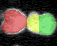
\includegraphics[width=\scalingfactor\textwidth]{images/joint/78_seg_crop.png}}
        };
        \begin{pgfonlayer}{upper}
            \begin{scope}[every node/.append style={scale=0.7}]
                \node[fg_det, label={[font=\tiny]center:$X_1^t$}] (a1) at (image1.south east) {};
                \node[fg_det, label={[font=\tiny]center:$X_2^t$}] (a2) at ($(image1.south east)!0.5!(image1.north east)$) {};
                \node[fg_det, label={[font=\tiny]center:$X_3^t$}] (a3) at (image1.north east) {};
                \node[fg_det, label={[font=\tiny]center:$X_5^t$}] (a5) at ($(image1.south west)!0.5!(image1.north west)$) {};
                \node[fg_det, label={[font=\tiny]center:$X_4^t$}] (a4) at ($(a3)!0.5!(a5)$) {};
            \end{scope}
            \begin{scope}[every node/.append style={scale=0.65}]
                \node[conflict,yshift=-5] (c1) at ($(a1)!0.5!(a5)$) {};
                \node[conflict, right=of a3, xshift=-10, yshift=-10] (c2) {};
                \node[conflict, yshift=-20] (c3) at (a4) {};
                \node[count, yshift=-20] (c4)  at ($(a2)!0.5!(a4)$) {};
                
                \path[count] (a1) edge (c4);
                \path[count] (a2) edge (c4);
                \path[count] (a3.south) edge (c4);
                \path[count] (a4) edge (c4);
                \path[count] (a5) edge[bend right=20] (c4);
                
                \path[conflict] (a5) edge[bend right=10] (c1);
                \path[conflict] (a1) edge (c1);

                \path[conflict] (a2) edge (c2);
                \path[conflict] (a4) edge[bend left=50] (c2);
                \path[conflict] (a5) edge[bend left=65] coordinate[pos=0.65](helpercoord1) (c2);

                \path[conflict] (a3) edge[bend left=10] (c3);
                \path[conflict] (a4) edge (c3);
                \path[conflict] (a5) edge (c3);
            \end{scope}
        \end{pgfonlayer}
        \begin{pgfonlayer}{bgupper}
            \node[rectangle, color=black,thick, fill=hypothesesbackground!30, opacity=0.8, draw=black,
            fit=(a1) (c2) (a5) (helpercoord1), inner sep=2, opacity=0.8, label={[xshift=5]above:{}}]
            (bgup) {};
        \end{pgfonlayer}
    \end{scope}
\end{scope}


%%% Local Variables: 
%%% mode: latex
%%% TeX-master: "../../main"
%%% End: 
